
%(BEGIN_QUESTION)
% Copyright 2007, Tony R. Kuphaldt, released under the Creative Commons Attribution License (v 1.0)
% This means you may do almost anything with this work of mine, so long as you give me proper credit

This paint mixing system mixes (clear) base and (colored) pigment to achieve a desired coloring, according to the ratio setpoint:

$$\includegraphics[width=15.5cm]{i01999x01.eps}$$

Determine what will happen to the paint's color over time if the base flowmeter turbine seizes so that it does not turn even when there is adequate flow through the pipe.  Also, explain {\it why} the paint's color will be affected as you predict.

\vskip 20pt \vbox{\hrule \hbox{\strut \vrule{} {\bf Suggestions for Socratic discussion} \vrule} \hrule}

\begin{itemize}
\item{} For those who have studied flow measurement, explain how a turbine flowmeter functions.
\item{} Explain what would happen in this process if the base control valve failed fully shut.
\item{} Explain what would happen in this process if the base control valve failed wide-open.
\item{} Explain what would happen in this process if the pigment control valve failed fully shut.
\item{} Explain what would happen in this process if the pigment control valve failed wide-open.
\item{} Explain what would happen in this process if the pigment flow controller (FC) were switched from remote setpoint to local setpoint.
\end{itemize}

\underbar{file i01999}
%(END_QUESTION)





%(BEGIN_ANSWER)


%(END_ANSWER)





%(BEGIN_NOTES)

The paint will become less and less colored over time, as the control system shuts off the flow of pigment entirely.  This will happen because the ratio control system sees no base flow anymore, and thus turns off the pigment flow to match.

%INDEX% Control, strategies: ratio

%(END_NOTES)


